
\section{Technical Overview of Our Approach}
\label{sec:techOverview}

\begin{figure*}[t]
  \centering
  

\tikzset{every picture/.style={line width=0.75pt}} %set default line width to 0.75pt        

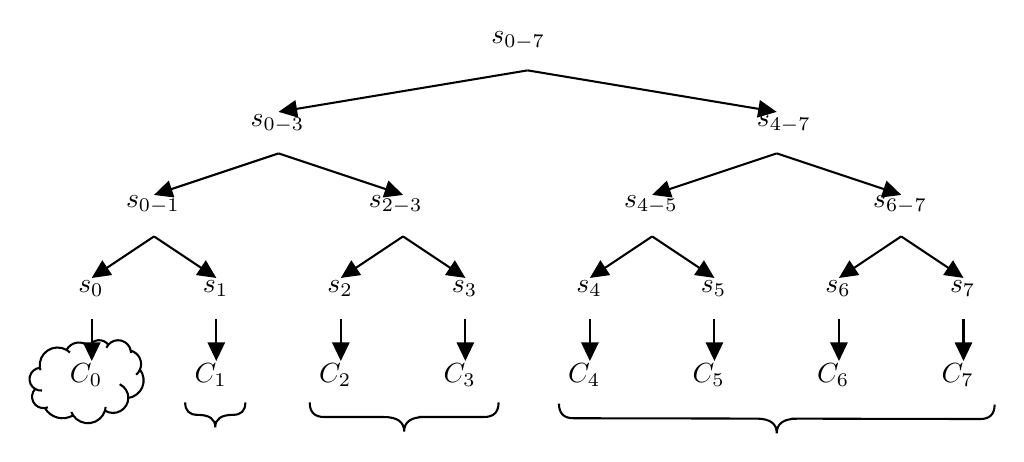
\begin{tikzpicture}[x=0.75pt,y=0.75pt,yscale=-1,xscale=1]
%uncomment if require: \path (0,300); %set diagram left start at 0, and has height of 300

%Straight Lines [id:da6211885505100274] 
\draw    (112.5,168.34) -- (140,150) ;
\draw [shift={(110,170)}, rotate = 326.31] [fill={rgb, 255:red, 0; green, 0; blue, 0 }  ][line width=0.08]  [draw opacity=0] (8.93,-4.29) -- (0,0) -- (8.93,4.29) -- cycle    ;
%Straight Lines [id:da045344571187413196] 
\draw    (140,150) -- (167.5,168.34) ;
\draw [shift={(170,170)}, rotate = 213.69] [fill={rgb, 255:red, 0; green, 0; blue, 0 }  ][line width=0.08]  [draw opacity=0] (8.93,-4.29) -- (0,0) -- (8.93,4.29) -- cycle    ;
%Straight Lines [id:da30999351200098524] 
\draw    (232.5,168.34) -- (260,150) ;
\draw [shift={(230,170)}, rotate = 326.31] [fill={rgb, 255:red, 0; green, 0; blue, 0 }  ][line width=0.08]  [draw opacity=0] (8.93,-4.29) -- (0,0) -- (8.93,4.29) -- cycle    ;
%Straight Lines [id:da0038108532391990524] 
\draw    (260,150) -- (287.5,168.34) ;
\draw [shift={(290,170)}, rotate = 213.69] [fill={rgb, 255:red, 0; green, 0; blue, 0 }  ][line width=0.08]  [draw opacity=0] (8.93,-4.29) -- (0,0) -- (8.93,4.29) -- cycle    ;
%Straight Lines [id:da5202996112606035] 
\draw    (352.5,168.34) -- (380,150) ;
\draw [shift={(350,170)}, rotate = 326.31] [fill={rgb, 255:red, 0; green, 0; blue, 0 }  ][line width=0.08]  [draw opacity=0] (8.93,-4.29) -- (0,0) -- (8.93,4.29) -- cycle    ;
%Straight Lines [id:da44817423034007153] 
\draw    (380,150) -- (407.5,168.34) ;
\draw [shift={(410,170)}, rotate = 213.69] [fill={rgb, 255:red, 0; green, 0; blue, 0 }  ][line width=0.08]  [draw opacity=0] (8.93,-4.29) -- (0,0) -- (8.93,4.29) -- cycle    ;
%Straight Lines [id:da1464427855443573] 
\draw    (472.5,168.34) -- (500,150) ;
\draw [shift={(470,170)}, rotate = 326.31] [fill={rgb, 255:red, 0; green, 0; blue, 0 }  ][line width=0.08]  [draw opacity=0] (8.93,-4.29) -- (0,0) -- (8.93,4.29) -- cycle    ;
%Straight Lines [id:da13582204926626829] 
\draw    (500,150) -- (527.5,168.34) ;
\draw [shift={(530,170)}, rotate = 213.69] [fill={rgb, 255:red, 0; green, 0; blue, 0 }  ][line width=0.08]  [draw opacity=0] (8.93,-4.29) -- (0,0) -- (8.93,4.29) -- cycle    ;
%Straight Lines [id:da30615324718513515] 
\draw    (142.85,129.05) -- (200,110) ;
\draw [shift={(140,130)}, rotate = 341.57] [fill={rgb, 255:red, 0; green, 0; blue, 0 }  ][line width=0.08]  [draw opacity=0] (8.93,-4.29) -- (0,0) -- (8.93,4.29) -- cycle    ;
%Straight Lines [id:da9271896843303857] 
\draw    (200,110) -- (257.15,129.05) ;
\draw [shift={(260,130)}, rotate = 198.43] [fill={rgb, 255:red, 0; green, 0; blue, 0 }  ][line width=0.08]  [draw opacity=0] (8.93,-4.29) -- (0,0) -- (8.93,4.29) -- cycle    ;
%Straight Lines [id:da09808697408042522] 
\draw    (382.85,129.05) -- (440,110) ;
\draw [shift={(380,130)}, rotate = 341.57] [fill={rgb, 255:red, 0; green, 0; blue, 0 }  ][line width=0.08]  [draw opacity=0] (8.93,-4.29) -- (0,0) -- (8.93,4.29) -- cycle    ;
%Straight Lines [id:da8331015133818496] 
\draw    (440,110) -- (497.15,129.05) ;
\draw [shift={(500,130)}, rotate = 198.43] [fill={rgb, 255:red, 0; green, 0; blue, 0 }  ][line width=0.08]  [draw opacity=0] (8.93,-4.29) -- (0,0) -- (8.93,4.29) -- cycle    ;
%Straight Lines [id:da898168093393371] 
\draw    (202.96,89.51) -- (320,70) ;
\draw [shift={(200,90)}, rotate = 350.54] [fill={rgb, 255:red, 0; green, 0; blue, 0 }  ][line width=0.08]  [draw opacity=0] (8.93,-4.29) -- (0,0) -- (8.93,4.29) -- cycle    ;
%Straight Lines [id:da13345957320943236] 
\draw    (320,70) -- (437.04,89.51) ;
\draw [shift={(440,90)}, rotate = 189.46] [fill={rgb, 255:red, 0; green, 0; blue, 0 }  ][line width=0.08]  [draw opacity=0] (8.93,-4.29) -- (0,0) -- (8.93,4.29) -- cycle    ;
%Straight Lines [id:da05876416812491858] 
\draw    (110,207) -- (110,190) ;
\draw [shift={(110,210)}, rotate = 270] [fill={rgb, 255:red, 0; green, 0; blue, 0 }  ][line width=0.08]  [draw opacity=0] (8.93,-4.29) -- (0,0) -- (8.93,4.29) -- cycle    ;
%Straight Lines [id:da5654275867640988] 
\draw    (170,207) -- (170,190) ;
\draw [shift={(170,210)}, rotate = 270] [fill={rgb, 255:red, 0; green, 0; blue, 0 }  ][line width=0.08]  [draw opacity=0] (8.93,-4.29) -- (0,0) -- (8.93,4.29) -- cycle    ;
%Straight Lines [id:da31932671168937365] 
\draw    (230,207) -- (230,190) ;
\draw [shift={(230,210)}, rotate = 270] [fill={rgb, 255:red, 0; green, 0; blue, 0 }  ][line width=0.08]  [draw opacity=0] (8.93,-4.29) -- (0,0) -- (8.93,4.29) -- cycle    ;
%Straight Lines [id:da11489740917816627] 
\draw    (290,207) -- (290,190) ;
\draw [shift={(290,210)}, rotate = 270] [fill={rgb, 255:red, 0; green, 0; blue, 0 }  ][line width=0.08]  [draw opacity=0] (8.93,-4.29) -- (0,0) -- (8.93,4.29) -- cycle    ;
%Straight Lines [id:da24817292659767398] 
\draw    (350,207) -- (350,190) ;
\draw [shift={(350,210)}, rotate = 270] [fill={rgb, 255:red, 0; green, 0; blue, 0 }  ][line width=0.08]  [draw opacity=0] (8.93,-4.29) -- (0,0) -- (8.93,4.29) -- cycle    ;
%Straight Lines [id:da5549995270865108] 
\draw    (410,207) -- (410,190) ;
\draw [shift={(410,210)}, rotate = 270] [fill={rgb, 255:red, 0; green, 0; blue, 0 }  ][line width=0.08]  [draw opacity=0] (8.93,-4.29) -- (0,0) -- (8.93,4.29) -- cycle    ;
%Straight Lines [id:da25264418335124195] 
\draw    (470,207) -- (470,190) ;
\draw [shift={(470,210)}, rotate = 270] [fill={rgb, 255:red, 0; green, 0; blue, 0 }  ][line width=0.08]  [draw opacity=0] (8.93,-4.29) -- (0,0) -- (8.93,4.29) -- cycle    ;
%Straight Lines [id:da07214105669651583] 
\draw    (530,207) -- (530,190) ;
\draw [shift={(530,210)}, rotate = 270] [fill={rgb, 255:red, 0; green, 0; blue, 0 }  ][line width=0.08]  [draw opacity=0] (8.93,-4.29) -- (0,0) -- (8.93,4.29) -- cycle    ;
%Shape: Cloud [id:dp5196949234271024] 
\draw   (85.01,213.17) .. controls (84.56,209.94) and (86.02,206.75) .. (88.75,204.95) .. controls (91.48,203.14) and (95.02,203.04) .. (97.85,204.68) .. controls (98.86,202.81) and (100.7,201.51) .. (102.81,201.19) .. controls (104.93,200.87) and (107.07,201.56) .. (108.6,203.05) .. controls (109.45,201.35) and (111.13,200.2) .. (113.04,200.02) .. controls (114.95,199.85) and (116.82,200.66) .. (117.98,202.17) .. controls (119.52,200.36) and (121.98,199.6) .. (124.29,200.22) .. controls (126.6,200.83) and (128.34,202.71) .. (128.77,205.03) .. controls (130.66,205.54) and (132.24,206.84) .. (133.09,208.6) .. controls (133.95,210.35) and (133.99,212.39) .. (133.22,214.18) .. controls (135.08,216.58) and (135.52,219.79) .. (134.36,222.6) .. controls (133.21,225.4) and (130.64,227.39) .. (127.61,227.82) .. controls (127.58,230.46) and (126.12,232.88) .. (123.79,234.15) .. controls (121.46,235.42) and (118.61,235.34) .. (116.35,233.94) .. controls (115.39,237.1) and (112.68,239.42) .. (109.4,239.91) .. controls (106.12,240.39) and (102.85,238.95) .. (101,236.21) .. controls (98.74,237.56) and (96.03,237.95) .. (93.47,237.29) .. controls (90.92,236.63) and (88.74,234.97) .. (87.43,232.7) .. controls (85.12,232.97) and (82.88,231.78) .. (81.83,229.73) .. controls (80.78,227.68) and (81.14,225.19) .. (82.73,223.52) .. controls (80.67,222.31) and (79.62,219.93) .. (80.13,217.6) .. controls (80.63,215.28) and (82.58,213.54) .. (84.96,213.29) ; \draw   (82.73,223.52) .. controls (83.71,224.08) and (84.83,224.34) .. (85.95,224.25)(87.43,232.7) .. controls (87.91,232.64) and (88.38,232.52) .. (88.84,232.35)(101,236.21) .. controls (100.66,235.71) and (100.38,235.16) .. (100.15,234.6)(116.35,233.94) .. controls (116.53,233.37) and (116.64,232.77) .. (116.69,232.17)(127.6,227.82) .. controls (127.63,225.02) and (126.02,222.45) .. (123.47,221.22)(133.22,214.18) .. controls (132.8,215.13) and (132.17,215.98) .. (131.38,216.66)(128.77,205.03) .. controls (128.84,205.42) and (128.87,205.81) .. (128.86,206.2)(117.98,202.17) .. controls (117.59,202.62) and (117.28,203.12) .. (117.04,203.66)(108.6,203.05) .. controls (108.39,203.45) and (108.24,203.89) .. (108.14,204.33)(97.85,204.68) .. controls (98.45,205.03) and (99.01,205.45) .. (99.51,205.93)(85.01,213.17) .. controls (85.07,213.61) and (85.16,214.05) .. (85.29,214.48) ;
%Shape: Brace [id:dp37789584804120313] 
\draw   (335.1,230.59) .. controls (335.09,235.26) and (337.41,237.59) .. (342.08,237.6) -- (430.03,237.77) .. controls (436.7,237.78) and (440.03,240.12) .. (440.02,244.79) .. controls (440.03,240.12) and (443.36,237.8) .. (450.03,237.81)(447.03,237.8) -- (537.99,237.98) .. controls (542.66,237.99) and (544.99,235.66) .. (545,230.99) ;
%Shape: Brace [id:dp3826911569900966] 
\draw   (215,230) .. controls (215,234.67) and (217.33,237) .. (222,237) -- (250.5,237) .. controls (257.17,237) and (260.5,239.33) .. (260.5,244) .. controls (260.5,239.33) and (263.83,237) .. (270.5,237)(267.5,237) -- (299,237) .. controls (303.67,237) and (306,234.67) .. (306,230) ;
%Shape: Brace [id:dp8696613256451281] 
\draw   (155,230) .. controls (155,233.98) and (156.99,235.97) .. (160.97,235.97) -- (160.97,235.97) .. controls (166.66,235.97) and (169.5,237.96) .. (169.5,241.94) .. controls (169.5,237.96) and (172.34,235.97) .. (178.03,235.97)(175.47,235.97) -- (178.03,235.97) .. controls (182.01,235.97) and (184,233.98) .. (184,230) ;

% Text Node
\draw (98,209.93) node [anchor=north west][inner sep=0.75pt]   [align=left] {$\displaystyle C_{0}$};
% Text Node
\draw (218,209.93) node [anchor=north west][inner sep=0.75pt]   [align=left] {$\displaystyle C_{2}$};
% Text Node
\draw (278,209.93) node [anchor=north west][inner sep=0.75pt]   [align=left] {$\displaystyle C_{3}$};
% Text Node
\draw (338,209.93) node [anchor=north west][inner sep=0.75pt]   [align=left] {$\displaystyle C_{4}$};
% Text Node
\draw (398,209.93) node [anchor=north west][inner sep=0.75pt]   [align=left] {$\displaystyle C_{5}$};
% Text Node
\draw (458,209.93) node [anchor=north west][inner sep=0.75pt]   [align=left] {$\displaystyle C_{6}$};
% Text Node
\draw (518,209.93) node [anchor=north west][inner sep=0.75pt]   [align=left] {$\displaystyle C_{7}$};
% Text Node
\draw (102,169.93) node [anchor=north west][inner sep=0.75pt]   [align=left] {$\displaystyle s_{0}$};
% Text Node
\draw (162,169.93) node [anchor=north west][inner sep=0.75pt]   [align=left] {$\displaystyle s_{1}$};
% Text Node
\draw (222,169.93) node [anchor=north west][inner sep=0.75pt]   [align=left] {$\displaystyle s_{2}$};
% Text Node
\draw (282,169.93) node [anchor=north west][inner sep=0.75pt]   [align=left] {$\displaystyle s_{3}$};
% Text Node
\draw (342,169.93) node [anchor=north west][inner sep=0.75pt]   [align=left] {$\displaystyle s_{4}$};
% Text Node
\draw (402,169.93) node [anchor=north west][inner sep=0.75pt]   [align=left] {$\displaystyle s_{5}$};
% Text Node
\draw (462,169.93) node [anchor=north west][inner sep=0.75pt]   [align=left] {$\displaystyle s_{6}$};
% Text Node
\draw (522,169.93) node [anchor=north west][inner sep=0.75pt]   [align=left] {$\displaystyle s_{7}$};
% Text Node
\draw (125,128.93) node [anchor=north west][inner sep=0.75pt]   [align=left] {$\displaystyle s_{0-1}$};
% Text Node
\draw (242,128.93) node [anchor=north west][inner sep=0.75pt]   [align=left] {$\displaystyle s_{2-3}$};
% Text Node
\draw (365,128.93) node [anchor=north west][inner sep=0.75pt]   [align=left] {$\displaystyle s_{4-5}$};
% Text Node
\draw (485,128.93) node [anchor=north west][inner sep=0.75pt]   [align=left] {$\displaystyle s_{6-7}$};
% Text Node
\draw (185,89.93) node [anchor=north west][inner sep=0.75pt]   [align=left] {$\displaystyle s_{0-3}$};
% Text Node
\draw (429,89.93) node [anchor=north west][inner sep=0.75pt]   [align=left] {$\displaystyle s_{4-7}$};
% Text Node
\draw (301,49.93) node [anchor=north west][inner sep=0.75pt]   [align=left] {$\displaystyle s_{0-7}$};
% Text Node
\draw (158,209.93) node [anchor=north west][inner sep=0.75pt]   [align=left] {$\displaystyle C_{1}$};


\end{tikzpicture}

  \caption{%
    Suppose there are $8$ branches $\cir_0$ through $\cir_7$, and
    suppose \E guesses that $\cir_0$ is the taken branch.
    If the taken branch is in the subtree $\cir_4$ through $\cir_7$,
    \E will generate the same garbage material for the entire subtree,
    regardless of which branch is actually taken.
    By extension, $\cir_0$ can only be evaluated against $\log 8 = 3$ garbage
    material strings: one for each sibling subtree (sibling subtrees
    are bracketed). Hence $\cir_0$ has only three possible sets of
    garbage output labels.
  }\label{fig:seed-tree}
\end{figure*}

We now informally present our construction with sufficient detail to introduce
the most interesting technical challenges and solutions.

\subsection{$O(b\log b)$ Stacked Garbling}
\label{sec:techOverviewSG}

Our main contribution is the reduction of SGC computation
from $O(b^2)$ to $O(b \log b)$.  Our constants are also
low: together \G and \E make a total of $\frac{5}{2} b \log b + b$ calls to \Gb\
and $b\log b + b$ calls  to \Ev.

We continue the discussion from~\Cref{sec:intuition} in more detail.
Our main task is the garbage collection of output labels of {\em
incorrectly guessed} $(\truth, \guess)$ combinations 
%w.r.t. taken (active) branch, 
where
\guess is \E's guess of the active branch, and \truth defines the active branch w.r.t. \guess.
Wlog, let $b$ be a power of $2$ to simplify notation.
Consider a binary tree where the leaves are the $b$ branches
$\cir_0,...,\cir_{b-1}$.  The tree provides an infrastructure to group branches and to unify processing.


Fix one of $b$ choices for \guess.  In contrast with~\HK, which then considers $b$ choices for \truth independently from \guess, we define \truth\ {\em in relation} to \guess, and consider fewer \truth options.
Namely,
% for each tree level $i$, 
we  let \truth  denote the sibling subtree of \guess that contains the
active branch (cf. notation~\Cref{sec:intuition}). 
Given a fixed incorrect \guess, there are only $\log b$ choices for
\truth.\footnote{We focus on garbage collection and
consider only incorrect guesses;  managing output labels of the correctly guessed branches is straightforward and cheap.}
While we have redefined \truth, the active branch ID \aid\ continues
to point to the single active branch.
%
Our garbled gadgets compute functions of \aid.
% In contrast to \HK, where \truth\ and the active branch ID \aid\ are
% the same, our \truth\ is a subtree \emph{containing} \aid.

For concreteness,
%in our discussion we 
consider the illustrative example of an $8$-leaf tree in~\Cref{fig:seed-tree} where $\guess=0$. 
The discussion and arguments pertaining to this special case generalize to arbitrary $b$ and $\guess$.

Consider the four scenarios where one of the branches $\cir_4-\cir_7$ is active.
These four scenarios each correspond
to $\truth = 1$: $\cir_4-\cir_7$ all belong to the level-$1$ sibling subtree of
$\cir_0$.
%
We ensure that \E's unstacking and evaluation in each
of these four cases is \emph{identical}, and hence she evaluates the
same garbage output labels in these four cases.  More generally, we achieve identical processing for all leaves of each sibling subtree.
Let \aid\ denote the index of the active branch. That is, \aid\ is a $\log
b$-bit integer that points to the active branch.
% To achieve our objective, \E will use garbled labels corresponding to
% \aid to compute seeds for the various nodes in the tree.

% Recall, as part of GC  evaluation, \aid is computed by the circuit, and \E obtains the corresponding $ \log b$-long vector of GC labels $\vec S$, where
% $S[i] \in \{S^0[i],S^1[i]\}$; \G of course knows all labels $S^0[i],S^1[i]$.

\subsubsection{Actions and gadgets of \G.}

\begin{figure}[t!]\centering\framebox{%
\begin{minipage}{1.05\linewidth}
\begin{itemize}
  \item \textsc{Inputs:} \gadget takes as input the active branch id
    \aid\ and
    the number of branches $b$.
  \item \textsc{Outputs:}
    \gadget outputs a sequence of evaluator seeds that form a binary branching tree:
  \[
    \es_{0, b-1}, \es_{0, \frac{b-1}{2}}, \es_{\frac{b-1}{2}+1,b-1},
    \ldots, \es_0, \es_1,\ldots \es_{b-1}
  \]
    such
    that for each node \node:
   \[
   \es_\node =
   \begin{cases}
     s_\node,& \text{if $\node$ is a sibling root of $\aid$}\\
     s_\node',& \text{otherwise}
   \end{cases}
  \]
  where $s_\node'$ is a uniform string indistinguishable from
  $s_\node$.
\end{itemize}
\end{minipage}
}\caption{%
  The \gadgetlong functionality. \gadgetlong is
  responsible for conveying only the sibling root seeds of \aid\ to \E.
  For every other node, \E obtains a different, but indistinguishable,
  seed that, when garbled, generates garbage material.
  %
  \gadgetlong is easily implemented as a garbled circuit gadget (i.e.,
  built from garbled rows).
}\label{fig:sortinghat}
\end{figure}

In the context of the example in~\Cref{fig:seed-tree}, \G  garbles
branches  $\cir_0,...,\cir_7$ as follows.
Recall, the active branch ID \aid\ is available to \G\ in form of
garbled labels.
% Given the labels corresponding to the active branch ID \aid,
\G chooses a random
seed for the root of the tree (denoted $s_{0,7}$ for the $8$-leaf tree
in~\Cref{fig:seed-tree}), and uses it to pseudorandomly derive seeds
for each node of the tree.  This is done in the standard manner, e.g.,
the immediate children of a seed $s$ are the PRF evaluations on inputs
$0$ and $1$ with the key $s$.
\G uses each leaf seed $s_i$ to garble the corresponding branch $\cir_i$ and stacks all garbled branches $\mat=\bigoplus_i \gcir_i$.  
%
This material $\mat$ is the large string that \G\ ultimately sends
across the network to \E.
We note two facts about $\mat$ and about the active branch $\aid$.
\begin{enumerate}
  \item \textbf{Correctness}: if \E\ obtains the $\log b$ seeds of the
    sibling roots of
    $\aid$, then she can regarble all circuits $\gcir_{i\neq \act}$,
    unstack by XORing with \mat, and obtain $\gcir_\act$, allowing her to
    correctly evaluate $\cir_\act$.
  \item \textbf{Security}: \E\ must not obtain any correct seed
    corresponding to any ancestor of \aid. If she did, she would learn (by garbling) the
    encoding of wire labels which would allow her to decrypt all
    intermediate wire values in $\cir_\act$.
    %
    Instead, \E\ will obtain `garbage' seeds indistinguishable yet
    distinct from the correct seeds generated by \G.
\end{enumerate}

To facilitate secure garbled evaluation of the conditional and meet the requirements of these two facts, in addition to \mat,
\G  generates and sends to \E a small (linear in the
number of branches with small constants) garbled gadget
that we call \gadget.\footnote{%
  In J.K. Rowling's Harry Potter universe, the `sorting hat' is a
  magical object that assigns new students to different school houses
  based on personality.
  Our \gadget\ `sorts' nodes of trees into two categories based on
  \aid: those that
  are `good' (i.e., sibling roots of the active branch) and those that
  are `bad'.
}
\gadget aids \E in her secure reconstruction of branch material. 
Specifically, \gadget takes as input labels corresponding to \aid\ and
produces candidate seeds for each node in the tree.
For each node \node, \gadget constructs a correct (i.e. as generated by \G) seed $s_\node$
if and only if \node is a sibling root  of the leaf \aid.
\gadget can easily be implemented as a collection of garbled rows.
Importantly, since this is a fixed
gadget, when evaluated on a node \node that is not a sibling root of
\aid, \E will obtain a {\em single} predictable to \G\ fixed garbage
seed. 
% We need to ensure this garbage value is the same for every
% \aid. This is easy to do.  Details follow:

For example in~\Cref{fig:seed-tree}, if the active branch is $\aid=4$,
then applying \gadget\ to nodes $\node_{0,3}, \node_{6,7},
\node_{5}$ will reconstruct the correct seeds $s_{0,3}, s_{6,7}, s_{5}$.  Applying \gadget to other nodes
will construct fixed garbage seeds.
If the active branch were instead $\aid=3$, then \gadget
would reconstruct the correct seeds $s_{4,7}, s_{0,1}, s_{2}$.
Critically, the
garbage seeds reconstructed
in both cases, e.g. for node $\node_{4,5}$, are the same.


\subsubsection{Actions of \E.}

It is now intuitive how \E proceed with unstacking. 
She applies \gadget and obtains a tree of random-looking seeds; of $2b$
seeds, only $\log b$ seeds just off the path to \aid\ (corresponding
to \aid's sibling roots) are correct.  \E guesses \guess; assuming
\guess, she uses only the sibling seeds of \guess to derive all
$b-1$ leaf seeds not equal to \guess.  She then garbles the $b-1$
branches $\cir_i$ and unstacks the corresponding GCs $\gcir_i$.

Clearly, if $\guess=\aid$, \E\ derives the intended leaf seeds
$s_{i\neq\aid}$, unstacks the intended garbled circuits
$\gcir_{i\neq\aid}$, and obtains the correct GC $\gcir_\aid$.
%
Consider the case where \E\ guesses wrong. %Firstly, there is no security violation since she will never receive any additional valid seeds;
\E simply unstacks wrong branches garbled with the wrong seeds.
Since \E never receives any additional valid seeds,
there is no security loss.  We next see that the number of different
garbage labels we must collect is small, and further that they can be
collected efficiently.

\subsubsection{Computational cost accounting.} Let's now verify that
we indeed reduced the number of calls to \Gb\ and \Ev\ to $O(b \log
b)$.  This is easily done by first considering how many such calls are
made by \E.  Consider branch $\cir_i$.  It is garbled $\log b$ times,
once with a seed (ultimately) derived from each seed on the path to
the root.  Thus, total number of calls by \E to \Gb\ is $b \log b$ and
to \Ev\ is exactly $b$.  

To construct the garbage collecting multiplexer, \G must obtain all possible garbage labels.  We
demonstrate that the total cost to the generator is $b (\log b +
1)$ calls to \Gb\ and $b \log b$ calls to \Ev.
First, consider only \Gb\ and consider the number of ways \E\ can garble a specific circuit $\cir_i$. Clearly, this is exactly $\log b+1$.

Now, consider the number of calls needed to \Ev.  Recall that our
goal was to ensure that \E constructs the same garbage output labels
for a branch $\cir_i$ in each scenario where \aid\ is in some fixed
sibling subtree of $\cir_i$. Note that the logic of \gadget\ ensures
that \E obtains the same sibling root seeds in each of these
scenarios, and therefore she constructs the same garblings. Hence,
since there are $\log b$ sibling subtrees of $\cir_i$, $\cir_i$ has
only $\log b$ possible garbage output labels.
Thus, in order to emulate \E\ in all settings and obtain all possible
garbage output labels, \G\ must garble and evaluate each branch $\log b$ times.


\subsection{Technical difference between our and~\HK binary braching}
\label{sec:techOverviewDiff}

A careful reader familiar with~\HK may notice that they present two
versions of stacked garbling.
The first handles high branching factors by recursively \emph{nesting}
conditionals.
Nested conditionals can be viewed as a binary branching
tree.
This first approach is then discarded in favor of a second, more efficient vector approach.
Our work advocates binary branching and yet substantially improves
over~\HK's vectorized approach.
Why is our binary branching better?

The problem with~\HK's recursive construction
is that the evaluator \E recursively garbles the garbage collecting multiplexer for
nested sub-conditionals.
However, doing so leads to a recursive emulation whereby \E
emulates herself (and hence \G emulates himself as well).
This recursion leads to quadratic cost for both players.
The way out is to treat the multiplexer separately, and to opt not
to stack it.
If multiplexers are not stacked, then \E need not garble them, and
hence \E\ need never emulate herself.
On top of this, we reduce the number of ways that individual branches
can be garbled via our \gadget.

\subsubsection{A note on nested branches.}
Nesting branches may seem desirable. Indeed, nested branches with
complex sequencing of instructions emerge
naturally in many programs.
%
Our approach operates directly over vectors of circuits and treats
them as binary branching trees.
This may at first seem like a disadvantage, since at the
time the first nested branching decision is made, it may not yet be
possible to make \emph{all} branching decisions.
%
There are two natural ways \ourschemelong\ can be used in such
contexts:
%
\begin{enumerate}
  \item Although we advocate for vectorized branching,
    \ourschemelong\ does support nested evaluation.
    More precisely, \ourschemelong\ handles branches by passing them
    to another \emph{underlying
    garbling scheme}, and it is secure to instantiate this underlying
    scheme with \ourschemelong\ itself.
    Although this is secure and correct, we do not necessarily
    recommend it. Using \ourschemelong\ in this recursive manner
    yields quadratic computation overhead.
  \item Refactorings can be applied to ensure branches
    are vectorized. For example, consider the following refactoring:
    \begin{align*}
      &{ \tt if~(e_0)~\{~s_0 ;
      if~(e_1)~\{~s_1~\}~else~\{~s_2~\}~\}~else~\{~s_3 ; s_4~\}
    \longrightarrow}
    \\
      &~~{ \tt if~(e_0)~\{~s_0~\}~else~\{~s_3~\};
        switch (2e_0 + (1 \minus e_0)e_1)~\{~s1~\}~\mid~\{~s_2~\}~\mid~\{~s_4~\}
    }
    \end{align*}
    Where $s_i$ are programs, $e_i$ are predicates on program
    variables, and where $s_0, s_3$ do not modify variables in $e_0$.
    This refactoring has replaced a nested conditional by a sequence
    of two `vectorized' conditionals, and hence made the approach
    amenable to our efficient algorithms.
\end{enumerate}
%


\subsection{Memory Efficiency of \ourschemelong}
\label{sec:memoryEfficiency}

\vlad{TBD. explain why HK20 is bad and how we resolve}




\subsection{Stacked garbling with and without Random Oracles}
\label{sec:techOverviewRO}


% We eliminate the need for employing calls to RO in~\HK.   

\HK (and we)
focus only on branching and leave the handling of low level gates to
another \emph{underlying} garbling scheme, \underscheme.
\HK\ assumes nothing about \underscheme except that it satisfies the standard
\cite{CCS:BelHoaRog12} properties, as well as their {\em stackability} property.
Assuming only  these properties does not preclude \underscheme's
labels being related to each other, which presents problems in the
standard model. \HK handles the possible use of related keys by using
a RO to construct their garbled gadgets.

We introduce a stronger requirement on \underscheme, which we call {\em strong stackability}.  Informally, it additionally requires that {\em all} output labels of \underscheme used in key derivation look uniformly random.  We show that this is sufficient for security in the standard model.

Of course, RO-based security theorems and proofs also work (and we explicitly claim them), and our gadgets could be slightly optimized in a natural manner under this assumption.





